\documentclass[12pt,a4paper,oneside]{book}

\usepackage[utf8]{inputenc}
\usepackage[english]{babel}
\usepackage{amssymb}
\usepackage{frontespizio}
\usepackage{enumitem}
\usepackage{fancyhdr}
\usepackage{eurosym}
\usepackage{graphicx}
\usepackage{xcolor}
\usepackage{minted}
\usepackage{float}

\fancypagestyle{plain}{
	\fancyhf{}
	\fancyfoot[C]{\thepage}
	\renewcommand{\headrulewidth}{\ifnum\value{chapter}>0 0.5pt \else 0pt \fi}
	\renewcommand{\footrulewidth}{0pt}
	\fancyhead[L]{\ifnum\value{chapter}>0 \bfseries \itshape \nouppercase \leftmark \fi}
}

\pagestyle{plain}

\newcommand\itemtext[2]{
	\expandafter\gdef\csname item#1\endcsname{#2}
	\label{#1}#2}

\newcommand\refitemtext[1]{\csname item#1\endcsname}

\restylefloat{table}

\begin{document}
	
\begin{frontespizio}
	\Istituzione{Politecnico di Milano}
	\Logo[3cm]{logo.png}
	\Divisione{Computer Science and Engineering}
	\Scuola{}
	\Titoletto{Software Engineering 2}
	\Titolo{Design document}
	\Sottotitolo{\textbf{PowerEnJoy}}
	\NCandidato{Authors}
	\Candidato{Francesco Fabiani\\Jagadesh Manivannan\\Niccolò Pozzolini}
	\NRelatore{Professors}{}
	\Relatore{Elisabetta Di Nitto\\Luca Mottola}
	\Piede{Academic Year 2016/2017}
\end{frontespizio}
 
\tableofcontents

\chapter{Introduction}

\section{Purpose}
The Requirement Analysis and Specifications Document aims to provide in detail every aspect of the service PowerEnJoy, including its components, goals, constraints, functional and non-functional requirements. Use cases and scenarios for all the users involved will be provided as well to conform the product's objectives to the real world.

The last part of this document is reserved to the formalization of some features of the system involving the utilization of Alloy, a declarative specification language which provides a structural modeling tool based on first-order logic.

The high-level functionalities described in the RASD are intended for both developers and project managers. The former have to implement and test the functionalities while the latter must examine whether every requirement has been respected. It may also be useful to users in order to best take advantage of the service.

\section{Description of the problem}
The product described in this RASD is PowerEnJoy, a car-sharing service which offers to its users exclusively electric cars. It includes the common functionalities of its category: permitting to registered users to obtain the position of all the available cars, reserving one within a certain amount of time and continuously displaying the up-to-the-minute cost of the ride are just few of them. Moreover, PowerEnJoy stimulates users to behave virtuously towards the ecosystem by applying various types of discounts under specific conditions.

There are four software components that constitute the PowerEnJoy project. First, a back-end server provides APIs in order to simplify the communication related to the interactions of a user with the cars. Then two applications are available for a user to allow him/her the employment of every functionality: a web-based application (intended for visualization from desktop) and a mobile one. Lastly, every vehicle will be equipped with an on-board computer, used by the driver to manage the ride with the available options and see real-time information related to it, such as the time spent, the distance traveled and the total amount.

\section{Goals}
\begin{enumerate}[label={[G\arabic*]},labelindent=\parindent,leftmargin=*]
	\item \label{goal:registration} Registration of a user to the system
	\item \label{goal:cars_location} Finding the locations of the available cars
	\item \label{goal:reservation} Reservation of a car
	\item \label{goal:expiration} Expiration of reservation and penalization
	\item \label{goal:entry} Entry of registered user into the car
	\item \label{goal:charging} Start charging and notifying the registered user
	\item \label{goal:car_locking} Stop charging the registered user and lock the car
	\item \label{goal:safe_areas} Safe areas for parking the reserved cars
	\item \label{goal:passengers} Detection of extra passengers and applying discount
	\item \label{goal:battery} Detection of the battery status and applying discount
	\item \label{goal:special_areas} Detection of special parking areas and applying discount
	\item \label{goal:constraints} Checking parking and battery constraints and penalization
\end{enumerate}

\section{Domain properties}
\begin{itemize}
	\item User's data are always valid
	\item Location reported by the GPS is always accurate
	\item Every user can reserve just a car per time
\end{itemize}

\section{Glossary}

\subsection{Definitions}
\begin{itemize}
	\item \emph{Car}: electric vehicle provided by the service
	\item \emph{Guest} or \emph{Guest user}: person not registered to the service
	\item \emph{Registered user}: see \emph{User}
	\item \emph{Safe area}: set of parking spots where a user can leave a car without penalization 
	\item \emph{User}: person with a valid driving license registered to the service
\end{itemize}

\subsection{Acronyms}
\begin{itemize}
	\item \emph{API}: Application Programming Interface
	\item \emph{GPS}: Global Positioning System
	\item \emph{OS}: Operating System, related both to desktop and mobile platforms
	\item \emph{PIN}: Personal Identification Number
	\item \emph{RASD}: Requirements Analysis and Specification Document
	\item \emph{W3C}: World Wide Web Consortium
\end{itemize}

\section{Constrains}

\subsection{Regulatory policies}
While waiting for future conventions, at the moment toll and handicap parkings are forbidden. Timed parkings are also forbidden, since the user cannot ensure compliance with the deadline once left the car.

During the registration the system receive the user's permission to get his position and it has to handle sensible data according to the privacy law. To avoid SPAM the system can only use messages and notifications if strictly required to the proper operation of the system.

\subsection{Hardware limitations}
\begin{itemize}
	\item User's mobile device:
\begin{itemize}
	\item Connection speed \(\geqslant\) 3G
	\item GPS
	\item Enough memory available to install the app
\end{itemize}
	\item Car:
	\begin{itemize}
	\item GPS
	\item Weight sensor for each seat
	\item Fast Internet connection
	\item On-board computer with integrated system
\end{itemize}
\end{itemize}

\subsection{Interfaces to other applications}
Interface with an SMS gateway provider via standard SMS REST APIs, to verify the user's account and send important notifications.

\subsection{Parallel operation}
The server supports parallel reservations of cars from different users at the same time.

\section{Reference documents}
The Requirements Analysis and Specification Document has been composed following the indications and examples reported in the document ISO/IEC/ IEEE 29148, released by W3C, containing provisions for the processes and products related to the engineering of requirements for systems and software products and services throughout the life cycle.

With regards to the course named Software Engineering II and held by professors Luca Mottola and Elisabetta Di Nitto (Politecnico di Milano, a.~y. 2016/17), the document conforms to the guidelines provided during the lectures and within the material of the course.
\chapter{Integration strategy}

\section{Entry criteria}
This section shows the conditions that must be met before starting the integration in order to obtain significant results.

First, it is crucial that the RASD and DD documents are completely composed, so that a whole vision of the components of the system and their functionalities is available.

As regards the individual components, the development must go forward along with their unit testing, so that the new modules implemented do not interfere with the solidity if the system. For this reason, every component should have at least 90\% of its functionalities completed before the integration with other components is tested.

Moreover, the integration process should start when the following percentages of development are achieved:
\begin{itemize}
	\item 100\% of the database and availability helper components
	\item at least 80\% of the controller components
	\item at least 90\% of the payment components
	\item at least 50\% for the client application
\end{itemize}

The decision of requiring different amounts of functionalities according to the component is based on the order the integration will take place and on the time needed to accomplish the integration testing phase of each one.

\section{Elements to be integrated}

\section{Integration testing strategy}
The items to be tested consist of the integration of the code modules developed for the Power Enjoy project. For testing we choose the bottom-up approach. This means that integration testing starts at the bottom level.

Using the bottom-up approach, we will start integrating together those components that do not depend on other ones to work, or that only depend on already developed components. We chose this because the top level component when built has to be tested from the bottom level components in our project, i.e. we can simply say that it has few dependencies on the bottom level components for testing.

Moreover, working bottom-up allows us to follow more carefully the development process and the developers to start performing integration testing earlier in the development process as soon as the required components have been developed, so that parallelism and efficiency are maximized.

We want to test using the real values and functionalities. The integration tests described in this documents are at the component level. The integration tests of lower level code modules are described in the corresponding components unit test.

\section{Sequence of component/Function integration}
In this section we are going to describe the order of integration (and integration testing) of the various components and subsystems of Power Enjoy.
As a notation, an arrow going from component C1 to component C2 means that C1 is necessary for C2 to function and so it must have already been
implemented.

\subsection{Software integration sequence}
Following the already mentioned bottom-up approach, we now describe how
the various subcomponents are integrated together to create higher level
subsystems.

\subsubsection*{Database Management System}
The very basic elements that needs to be integrated and tested are Database and Availability Helper. We test this first because of the bottom up approach and
all the other subsystems components relies in this structure.

\subsubsection*{Controller System}
The second step is the integration of the components of the Controller System. Most of the important operations are assumed to be executed/performed
by the components of the controller system. We proceed further by showing which components are executed or integrated in sequence.

First, we proceed by integrating the Selection Controller with the database and Availability Helper.

\begin{figure}[h]
	\centering
	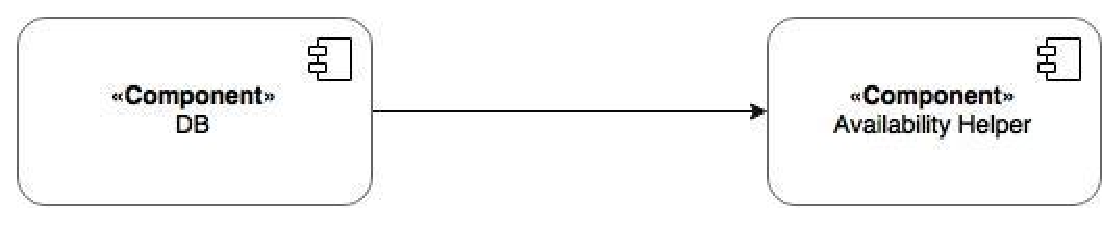
\includegraphics[height=1.4cm,keepaspectratio]{figures/itp1.eps}
	\label{fig:itp1}
\end{figure}

Then the same procedure is followed by replacing the selection controller with other components of the controller system in the following sequence: Reservation Controller, Ride controller, Parking Controller, Discount Controller.

\subsubsection*{Map Manager System}
Generally the communication between the controllers happens through the Map Manager. So, the Map Manager has to be integrated with the Controllers for their communication and also for interaction of the Client with the system.

\begin{figure}[h]
	\centering
	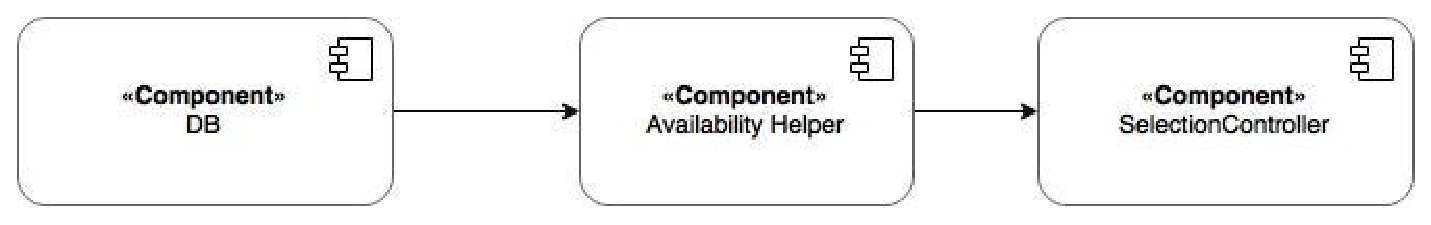
\includegraphics[height=1.4cm,keepaspectratio]{figures/itp2.eps}
	\label{fig:itp2}
\end{figure}

\begin{figure}[h]
	\centering
	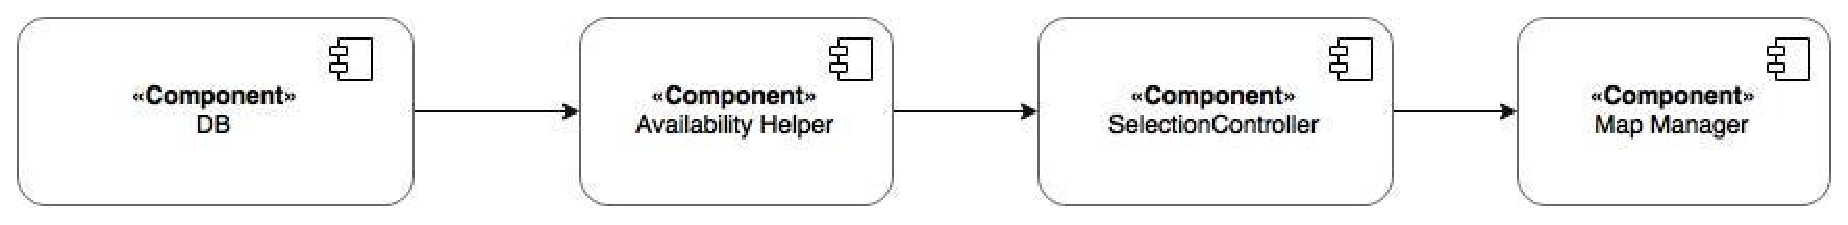
\includegraphics[height=1.4cm,keepaspectratio]{figures/itp3.eps}
	\label{fig:itp3}
\end{figure}

\subsubsection*{Notification System}
The next integration test is executed with the notification system. This notification system is developed by the third party and we just integrate and test here the functionalities. For example: after reserving a car, the user is notified with a confirmation acknowledgement.

\subsubsection*{Payment System}
\subsubsection*{Account Manager System}

\subsection{Subsystem integration sequence}
\chapter{Individual steps and test description}

In this chapter we are going to describe the tests that need to be executed for every couple of components which interact with each other. The integration between controllers is not tested because their interactions take place through the MapManager.

\section{Integration test case I1}
\begin{table}[h]
	\centering
	\begin{tabular*}{\textwidth}{p{4.4cm} @{\extracolsep{0.5cm}} p{8.5cm}}
		\hline
		\textbf{Test case identifier} & I1T1 \\
		\hline
		\textbf{Test item(s)} & Database \(\rightarrow\) Availability Helper \\
		\hline
		\textbf{Input specification} & Create typical SQL query (Database inputs) \\
		\hline
		\textbf{Output specification} & Check if the correct functions are called in the Availability Helper \\
		\hline
		\textbf{Environmental needs} & Necessary input parameters for testing \\
		\hline
	\end{tabular*}
\end{table}

\section{Integration test case I2}
\begin{table}[h]
	\centering
	\begin{tabular*}{\textwidth}{p{4.4cm} @{\extracolsep{0.5cm}} p{8.5cm}}
		\hline
		\textbf{Test case identifier} & I2T1 \\
		\hline
		\textbf{Test item(s)} & Availability Helper \(\rightarrow\) Selection Controller \\
		\hline
		\textbf{Input specification} & -- \\
		\hline
		\textbf{Output specification} & -- \\
		\hline
		\textbf{Environmental needs} & I1 succeeded \\
		\hline
	\end{tabular*}
\end{table}

\begin{table}[h]
	\centering
	\begin{tabular*}{\textwidth}{|p{4.cm}|p{8.86cm}|}
		\hline	
		\multicolumn{2}{|c|}{checkAvailability(zone)} \\
		\hline
		\textit{Input} & \textit{Effect} \\
		\hline
		A valid zone & Returns a list containing all the available cars in that zone \\
		\hline
		An invalid zone & An InvalidZoneException is generated \\
		\hline
		An null zone & A NullZoneException is generated \\
		\hline
	\end{tabular*}
\end{table}

\section{Integration test case I3}
\begin{table}[h]
	\centering
	\begin{tabular*}{\textwidth}{p{4.4cm} @{\extracolsep{0.5cm}} p{8.5cm}}
		\hline
		\textbf{Test case identifier} & I3T1 \\
		\hline
		\textbf{Test item(s)} &  Availability Helper \(\rightarrow\) Reservation Controller\\
		\hline
		\textbf{Input specification} & -- \\
		\hline
		\textbf{Output specification} & -- \\
		\hline
		\textbf{Environmental needs} & I1 succeeded \\
		\hline
	\end{tabular*}
\end{table}

\begin{table}[h]
	\centering
	\begin{tabular*}{\textwidth}{|p{4.cm}|p{8.86cm}|}
		\hline	
		\multicolumn{2}{|c|}{changeTagRequest(car, tag) returns response} \\
		\hline
		\textit{Input} & \textit{Effect} \\
		\hline
		A valid car and a valid tag & If parameter tag != old(car.tag) returns positive response. Otherwise an UnconsistentChangeException is generated (in this case most of the times it happens because someone else has been quicker than the user to reserve a car) \\
		\hline
		An invalid tag & An InvalidTagException is generated \\
		\hline
	\end{tabular*}
\end{table}

\newpage
\section{Integration test case I4}
\begin{table}[h]
	\centering
	\begin{tabular*}{\textwidth}{p{4.4cm} @{\extracolsep{0.5cm}} p{8.5cm}}
		\hline
		\textbf{Test case identifier} & I4T1 \\
		\hline
		\textbf{Test item(s)} & Availability Helper \(\rightarrow\) Parking Controller \\
		\hline
		\textbf{Input specification} & -- \\
		\hline
		\textbf{Output specification} & -- \\
		\hline
		\textbf{Environmental needs} & I1 succeeded \\
		\hline
	\end{tabular*}
\end{table}

\begin{table}[h]
	\centering
	\begin{tabular*}{\textwidth}{|p{4.cm}|p{8.86cm}|}
		\hline	
		\multicolumn{2}{|c|}{getSpecialParkingAreas(destination) returns SpecialParkingAreas} \\
		\hline
		\textit{Input} & \textit{Effect} \\
		\hline
		A valid destination & Returns a possibly empty SpecialParkingArea list \\
		\hline
		An invalid destination & An InvalidDestinationException is generated \\
		\hline
\end{tabular*}
\end{table}

\end{document}